\documentclass[]{article}
%\usepackage[a4paper, total={6.5in, 8.5in}]{geometry}
\usepackage{color}
\usepackage{hyperref}
\usepackage{amsmath}
\usepackage{amssymb}
\usepackage{graphicx}
\usepackage{float}
\usepackage{algorithm}
\usepackage{algpseudocode}
\usepackage{neurips_data_2023}

\title{Towards Comparable Active Learning}
\author{%
	David S.~Hippocampus\thanks{Use footnote for providing further information
		about author (webpage, alternative address)---\emph{not} for acknowledging
		funding agencies.} \\
	Department of Computer Science\\
	Cranberry-Lemon University\\
	Pittsburgh, PA 15213 \\
	\texttt{hippo@cs.cranberry-lemon.edu} \\
	% examples of more authors
	% \And
	% Coauthor \\
	% Affiliation \\
	% Address \\
	% \texttt{email} \\
	% \AND
	% Coauthor \\
	% Affiliation \\
	% Address \\
	% \texttt{email} \\
	% \And
	% Coauthor \\
	% Affiliation \\
	% Address \\
	% \texttt{email} \\
	% \And
	% Coauthor \\
	% Affiliation \\
	% Address \\
	% \texttt{email} \\
}

\begin{document}

\maketitle

\begin{abstract}
	The abstract paragraph should be indented $\frac{1}{2}$~inch (3~picas) on
	both the left- and right-hand margins. Use 10~point type, with a vertical
	spacing (leading) of 11~points.  The word \textbf{Abstract} must be centered,
	bold, and in point size 12. Two line spaces precede the abstract. The abstract
	must be limited to one paragraph.
\end{abstract}

\section{Introduction}
{\color{red} Version: Braindump}\\
Among others, the authors of \cite{zhou2021towards} have pointed out severe inconsistencies in results of AL papers in recent years. 
In their supplementary materials they conducted a meta analysis of reported results of several different AL algorithms and found that all considered algorithms only provided significant lifts in their own original papers, while all following literature reported performances no better that uncertainty sampling, or in some cases no better than random sampling for the same algorithm.
The result of these inconsistencies is a chaotic landscape of AL algorithms where every paper claims to archive state-of-the-art results by significantly outperforming everyone else, while the vast majority of results proves to be non-reproducible.

\subsection{Contributions}
\begin{enumerate}
	\item Evaluation of Active Learning algorithms on datasets from 4 different domains, including synthetic data that highlights principled shortcomings of existing approaches.
	\item Novel experimental protocol for seeding the experiment with 3 different seeds to allow full control and reproducibility and analysis of how many restarts are required to converge to the true median performance reliably.
	\item Simple algorithm for an Oracle-Curve that can be constructed greedily and does not rely on search.
\end{enumerate}

%%%%%%%%%%%%%%%%%%%%%%%%%%%%%%%%%%%%%%%%%%%%%%%%%%%%%%%%%%%%%%%%%%%%%%%%%%%%%%%%%%
\section{Related Work}
{\color{red} Version: Braindump}\\
Many different algorithms have been proposed for active learning. 
In this work we focus on those approaches that have shown consistent results over the years as well as newer approaches that have demonstrated significant lifts in their initial experiments.
AL algorithms can be categorized into two classes: Geometric approaches and uncertainty-based approaches.
Geometric approaches include CoreSet \cite{sener2017active} and TypiClust \cite{hacohen2022active}, which use clustering techniques to partition the data and then sample their unlabeled points based on the clusters.
Uncertainty-based approaches include classic uncertainty sampling (based on Shannon-Entropy and the margin-score), BALD \cite{kirsch2019batchbald} and BADGE \cite{ashdeep}, which use metrics to measure the classifiers state. \\ [1mm]
%
Some previous work also aimed to provide a benchmark suite for active learning:
The authors of \cite{beck2021effective} and \cite{li2022empirical} both focus on active learning in the image domain.
While \cite{beck2021effective} discuss a new metric to measure AL performance, which they call "Label Efficiency" and provide experiments on many common configurations for data preparation, model training and other hyperparameters, \cite{li2022empirical} focuses on combined approaches of AL and semi-supervised learning to aid model training.
The authors of \cite{hu2021towards} study models that are learned with AL techniques in the image and text domain.
They test for several different properties of the models including robustness, response to compression techniques and final performance.



%%%%%%%%%%%%%%%%%%%%%%%%%%%%%%%%%%%%%%%%%%%%%%%%%%%%%%%%%%%%%%%%%%%%%%%%%%%%%%%%%%
\section{Overview}
Table \ref{tab:benchmark_comparison} shows a feature comparison between our proposed benchmark and several existing benchmarks in the literature, as well as methodological AL papers with an extensive experiments section. \\
{\color{red} TODO} We include in this table any methodological paper that experiments on at least two domains. \\
{\color{red} TODO} Define AL scenarios (really hard)
\begin{table}[h]
	\centering
	\begin{tabular}{l | c c c c c}
		Paper & \# Datasets & Domains & Scenarios & Oracle & RL Alg. \\
		\hline
		Beck et al. \cite{beck2021effective} & 4 & 1 & 3 & - & - \\
		Hu et al. \cite{hu2021towards} & 5 & 2 & 1 & - & - \\
		Li et al. \cite{li2022empirical} & 5 & 1 & 1 & - & - \\
		Zhou et al. \cite{zhou2021towards} & 3 & 2 & 1 & \checkmark & - \\
		\textbf{Ours} & 5 & 2 & 2 & \checkmark & -
	\end{tabular}
	\caption{Comparison of our benchmark with the existing literature}
	\label{tab:benchmark_comparison}
\end{table}

%Manual NIPS Benchmark paper eval (out of 6):
%\begin{itemize}
%	\item Has new method: 1
%	\item Multiple domains: 2
%	\item $> 5$ datasets: 3
%	\item $> 5$ baselines: 4
%\end{itemize}


%%%%%%%%%%%%%%%%%%%%%%%%%%%%%%%%%%%%%%%%%%%%%%%%%%%%%%%%%%%%%%%%%%%%%%%%%%%%%%%%%%
\subsection{Problem Description}
{\color{red} Version: 1.0}\\
Given two spaces $\mathcal{X}:=\mathcal{R}^M$ and $\mathcal{Y}:=\mathcal{R}^C$, a sample $\mathcal{D}_1,\ldots,\mathcal{D}_N \subseteq (\mathcal{X}\times \mathcal{Y})^*$ of sequences of pairs $(x,y)$  from an unknown distribution $p$ called datasets and a number $B\in\mathcal{N}$ with $B < |\mathcal{D}|$. \\
Given two functions $\ell:\mathcal{Y}\times \mathcal{Y}\rightarrow \mathcal{R}$ called loss, and $A: (\mathcal{X} \times \mathcal{Y})^* \times \mathcal{X}^* \rightarrow \mathcal{Y}^{\mathcal{X}}$ called learning algorithm, find a function
\begin{align*}
	a: (\mathcal{X}\times \mathcal{Y})^* \times \mathcal{X}^* \rightarrow \{0,1\}^*
	\quad\quad \text{\tiny (equivariant in the second argument)}
\end{align*}
% which is equivariant in the second argument, 
called acquisition function, s.t. the expected loss of a model learned on all predictors plus $B$ acquired targets is minimal:
\begin{align*}
	\mathbb{E}_{\mathcal{D}\text{train},\mathcal{D}\text{test}\sim p}   &
	% \frac{1}{|\mathcal{D}\text{test}|} \sum_{(x,y)\in\mathcal{D}\text{test}}
	% \operatorname{avg} \{
	%  \ell(y, \hat y(x)) \mid (x,y)\in\mathcal{D}\text{test} \}
	\operatorname{avg}\limits_{(x,y)\in\mathcal{D}\text{test}}
	\ell(y, \hat y(x)) 
	\\
	\text{with }
	\hat y:= & A( (\mathcal{D}\text{train}_{n_1},\ldots,\mathcal{D}\text{train}_{n_B}), \mathcal{D}\text{train}|_{\mathcal{X}})
	\\ 
	n_b := & \text{index}( a( (\mathcal{D}\text{train}_{n_1},\ldots,\mathcal{D}\text{train}_{n_{b-1}}), \mathcal{D}\text{train}|_{\mathcal{X}}) ),
	\quad b\in 1{:}B
\end{align*}
(\textit{We would need to switch from lowest expected loss to highest AUC}) \\
Since combinatorial problem of finding the optimal subset $\mathcal{D}_\text{train}$ is computational not feasible, we allow sequential construction of $\mathcal{D}_\text{train}$. \\ [2mm]
%
To construct the active learning setting, we suppress the labels $\mathcal{Y}$ of $\mathcal{D}_\text{train}$ to form the unlabeled pool $\mathcal{U} := \mathcal{X}^*$ and form and initial labeled pool by uniformly sampling $k$ number of instances per class from $\mathcal{U}$ and recovering their label $\mathcal{L} := (\mathcal{X}, \mathcal{Y})^{k*C}$. \\ [2mm]

Following \cite{zhou2021towards}, the quality of an active learning algorithm is evaluated by an "anytime" protocol that incorporates classification performance at every iteration, not just the final performance after the budget is exhausted.
We employ the normalized area under the accuracy curve (AUC):
\begin{equation}\label{eq:auc}
	\operatorname{auc}(\mathcal{U}, \mathcal{L}, \hat y, B) := \frac{1}{B} \sum_{i=1}^{B} \operatorname{Acc}(y_{test}, \hat y_i(x_{test}))
\end{equation}
Where $\hat y_i$ is the retrained classification model after the i-\textit{th} instance was selected. \\ [1mm]
%
\textbf{Framing AL as RL}\\
We define the active learning process as an adapted reinforcement learning loop $(S, A, \tau, \Omega, \omega)$ where an environment iteratively will expose a state $s \in S$ to an agent $\Omega$, which will choose actions $a \in A$.
For each iteration $i$ the environment samples a subset of size $\tau$ of unlabeled instances $u^{(i)} \underset{\tau}{\sim} \mathcal{U}^{(i)}$, constructs the state $s^{(i)} := \omega(u^{(i)})$ and presents it to the agent to select an action $a^{(i)} := \Omega(s^{(i)})$.
The action $a^{(i)}$ is the index of the selected instance in $u^{(i)}$ out of all possible indices $A := [1 \ldots \tau]$.
This process is repeated $B$ times $i := [1 \ldots B]$.

% TODO: remove tau from pseudocode
\begin{minipage}{0.59\linewidth}
	\begin{algorithm}[H]
		\caption{Active Learning}\label{alg:active_learning}
		\begin{algorithmic}[1]
			\Require $\mathcal{U}$ \Comment{Unlabeled Pool}
			\Require $\tau$ \Comment{Unlabeled Sample Size}
			\Require $\Omega$ \Comment{AL Agent}
			\Require $\omega$ \Comment{Environment State function}
			\State $\mathcal{L}^{(1)} \gets \operatorname{seed}(\mathcal{U})$  \Comment{Create the initial labeled set}
			\State $\mathcal{U}^{(1)} \gets \mathcal{U}$
			\For{$i := 1 \ldots B$}
				\State $\text{acc}^{(i)} \gets \operatorname{Retrain}(\mathcal{L}^{(i)})$  %\Comment{$\operatorname{Retrain}(\mathcal{L}^{(i)})$ is shorthand for $\operatorname{Retrain}(\mathcal{L}^{(i)}, \mathcal{L}^\text{test}, \hat y_\theta, e^\text{max})$}
				\State $u^{(i)} \sim \text{unif}(1:|\mathcal{U}^{(i)}|)$
				\State $a^{(i)} \gets \Omega(u^{(i)}) \hspace{2mm}|\hspace{2mm} a \in 1:|u^{(i)}|$ 
				%\Comment{$a^{(i)}$ is an index inside of $u^{(i)}$}
				\State $y^{(i)} \gets \operatorname{label}(u^{(i)}_{a})$ 
				%\Comment{$u^{(i)}_{a}$ is shorthand for $u^{(i)}_{a^{(i)}}$}
				\State $\mathcal{L}^{(i+1)} \gets \mathcal{L}^{(i)} \cup \{(u^{(i)}_a, y^{(i)})\}$
				\State $\mathcal{U}^{(i+1)} \gets \mathcal{U}^{(i)} \setminus \{u^{(i)}_a\}$
			\EndFor
			\State
			\Return $\frac{1}{B} \sum_{i=1}^{B} \text{acc}^{(i)}$
		\end{algorithmic}
	\end{algorithm}
\end{minipage}
\hspace{3mm}
\begin{minipage}{0.35\linewidth}
	\begin{algorithm}[H]
		\caption{Retrain}\label{alg:retrain}
		\begin{algorithmic}[1]
			\Require $\mathcal{L}$ \Comment{Labeled Pool}
			\Require $\mathcal{L}^\text{test}$ \Comment{Labeled Test Data}
			\Require $\hat y_\theta$ \Comment{Classification Model}
			\Require $e^\text{max}$ \Comment{Maximum Epochs}
			\State $\text{loss}^* \gets \infty$
			\For{$i := 1 \ldots e^{\text{max}}$}
			\State $\theta_{i+1} \gets \theta_i - \eta \nabla_\theta \ell(\mathcal{L}, \hat y_{\theta})$
			\State $\text{loss}_i \gets \ell(\mathcal{L}^\text{test}, \hat y_{\theta})$
			\If{$\text{loss}_i < \text{loss}^*$}
			\State $\text{loss}^* \gets \text{loss}_i$
			\Else
			\State Break
			\EndIf
			\EndFor
			\State
			\Return Acc($\mathcal{L}^\text{test}, \hat y_{\theta}$)
		\end{algorithmic}
	\end{algorithm}
\end{minipage}


\begin{algorithm}
	\caption{Oracle}\label{alg:oracle}
	\begin{algorithmic}[1]
		\Require $\mathcal{U}$ \Comment{Unlabeled Pool}
		\Require $\tau$ \Comment{Unlabeled Sample Size}
		\Require $\Omega$ \Comment{AL Agent}
		\Require $\omega$ \Comment{Environment State function}
		\State $\mathcal{L}^{(1)} \gets \operatorname{seed}(\mathcal{U})$  \Comment{Create the initial labeled set}
		\State $\mathcal{U}^{(1)} \gets \mathcal{U}$
		\For{$i := 1 \ldots B$} 
			\State $\text{acc}^{(i)} \gets \operatorname{Retrain}(\mathcal{L}^{(i)})$  \Comment{$\operatorname{Retrain}(\mathcal{L}^{(i)})$ is shorthand for $\operatorname{Retrain}(\mathcal{L}^{(i)}, \mathcal{L}^\text{test}, \hat y_\theta, e^\text{max})$}
			\State $u^{(i)} \sim \text{unif}(1:|\mathcal{U}^{(i)}|)$
			\State $r* \gets -\infty$
			\State $j* \gets -1$
			\For{$j := 1 \ldots \tau$} \Comment{Testing every unlabeled point}
				\State $y^{(j)} \gets \operatorname{label}(u^{(i)}_{j})$
				\State $\mathcal{L}^{(j)} \gets \mathcal{L}^{(i)} \cup \{(u^{(i)}_j, y^{(j)})\}$
				\State $\text{acc}^{(j)} \gets \operatorname{Retrain}(\mathcal{L}^{(j)})$  
				\State $r^{(j)} \gets \text{acc}^{(j)} - \text{acc}^{(i)}$
				\If{$r^{(j)} > r^*$} \Comment{Select point with largest increase in performance}
					\State $r* \gets r^{(j)}$
					\State $j* \gets j$
				\EndIf  
			\EndFor
			\State $y^{(i)} \gets \operatorname{label}(u^{(i)}_{j*})$
			\State $\mathcal{L}^{(i+1)} \gets \mathcal{L}^{(i)} \cup \{(u^{(i)}_{j*}, y^{(i)})\}$
			\State $\mathcal{U}^{(i+1)} \gets \mathcal{U}^{(i)} \setminus \{u^{(i)}_{j*}\}$
		\EndFor
		\State
		\Return $\frac{1}{B} \sum_{i=1}^{B} \text{acc}^{(i)}$
	\end{algorithmic}
\end{algorithm}

%%%%%%%%%%%%%%%%%%%%%%%%%%%%%%%%%%%%%%%%%%%%%%%%%%%%%%%%%%%%%%%%%%%%%%%%%%%%%%%%%%
%%%%%%%%%%%%%%%%%%%%%%%%%%%%%%%%%%%%%%%%%%%%%%%%%%%%%%%%%%%%%%%%%%%%%%%%%%%%%%%%%%
%%%%%%%%%%%%%%%%%%%%%%%%%%%%%%%%%%%%%%%%%%%%%%%%%%%%%%%%%%%%%%%%%%%%%%%%%%%%%%%%%%
\section{Methodology}

%%%%%%%%%%%%%%%%%%%%%%%%%%%%%%%%%%%%%%%%%%%%%%%%%%%%%%%%%%%%%%%%%%%%%%%%%%%%%%%%%%
\subsection{Reproducibility}\label{sec:reproducibility}
{\color{red} Version: 1.0}\\
A big focus in this work is to provide an experimental setup that is fully reproducible independent from the dataset, classification model or AL algorithm used.
In our opinion, an evaluation on one dataset with a given seed should always be done on the same sequence of batches $x_0, \ldots, x_B$.
Even though different AL algorithms will pick different samples from these batches, making them unavailable for sampling in later batches, the theoretical decision tree for every possible choice in every iteration $i$ should stay the same.
This behavior is not possible with the default choice of setting a global seed at the start of the experiment, since a single additional random draw from the random number generator completely changes the decision tree for the batches.
This additional random number might be drawn during the initialization of the classification model, the AL algorithm, or even during every AL iteration if $\Omega$ is stochastic.
This problem also applies to the initialization of the classification model $\theta$, the initialization and querying of $\Omega$ and the drawn mini batches during the training of $\theta$.
The desired control over all these processes can be archived by assigning a separate seeded random number generator to all these processes.
To the best of our knowledge, we are the first work that discusses this issue and proposes a solution for it.
We hypothesize that the insufficient setup with global seeds contributes to the on-going problem of inconsistent results of AL algorithms in different papers. \\ [1mm]
In summary, we introduce three different seeds: $s_\Omega$ for the acquisition function, $s_\mathcal{D}$ for dataset splitting and mini batch sampling and $s_\theta$ for model initialization and sampling of dropout masks.
Unless stated otherwise, we will keep $s_\Omega$ fixed for restarts of the same experiment, while $s_\mathcal{D}$ and $s_\theta$ are incremented by 1 between restarts to introduce stochasticity into our framework.

%%%%%%%%%%%%%%%%%%%%%%%%%%%%%%%%%%%%%%%%%%%%%%%%%%%%%%%%%%%%%%%%%%%%%%%%%%%%%%%%%%
\subsection{Evaluation}\label{sec:evaluation}
{\color{red} Version: 1.0}\\
We compare different AL algorithms based on their median AUC score (Eq. \ref{eq:auc}) across multiple restarts of the experiment.
This score does incorporate performance in early stages (low budget) as well as capabilities to push the classifier in later stages (high budget).
A good AL algorithm should be able to perform well in both scenarios. \\ [1mm]
Since AUC is dependent on the chosen budget, we need a general rule on how to set this hyperparameter that does not inherently benefit a subset of algorithms.
In this work, we choose the budget per dataset to be the first point at which the oracle manages to reach a percentage of the upper bound performance.
Even though we would like to propose a single percentage value for all datasets, we found that different data modalities and use cases need different percentages to produce sensible budgets.
We propose the following values: \textbf{Tabular}: 99\%, \textbf{Image}: 90\% and \textbf{Text}: {\color{red}TODO}. \\ [1mm]
Additionally, we provide evidence in Fig. \ref{fig:restarts} that previous works have not evaluated their experiments with a sufficient number of restarts.
To create one slice in Fig. \ref{fig:restarts}, we used all our runs for the Splice dataset and drew multiple sub-sets of that respective size (X axis), effectively simulating an experiment with that many restarts.
Calculating the AUC values for every drawn run allows us to draw the box-plot.
Each box represents the variance of an evaluation if conducted with the respective number of restarts.
We can clearly observe that low repetitions ($<10$) provide an uncertain evaluation where lucky and unlucky draws of the same experiment give drastically different median AUC values.
\begin{figure}
	\centering
	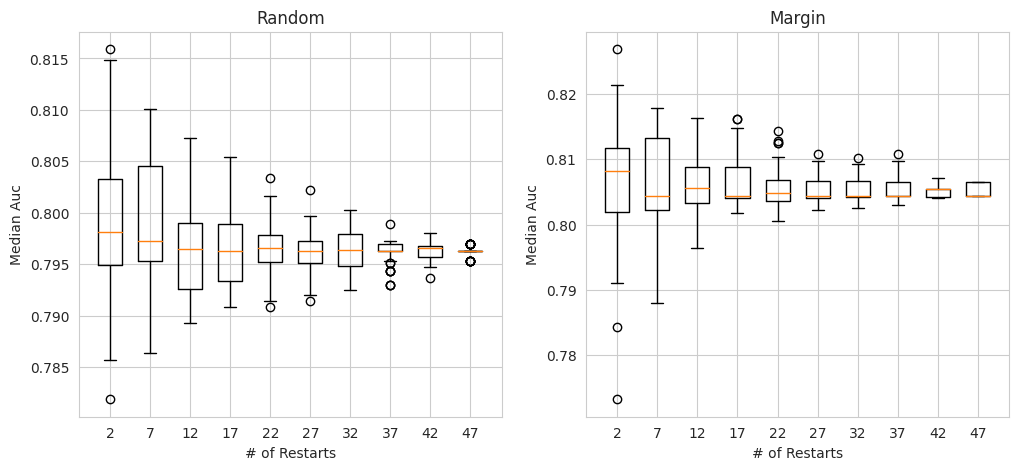
\includegraphics[width=\linewidth]{img/ablation_restarts.png}
	\caption{Random draws from Splice with different numbers of repetitions.}
	\label{fig:restarts}
\end{figure}
To combat is uncertain evaluation, we propose to repeat every experiment 50 times, to arrive at the true median AUC for each algorithm.

%%%%%%%%%%%%%%%%%%%%%%%%%%%%%%%%%%%%%%%%%%%%%%%%%%%%%%%%%%%%%%%%%%%%%%%%%%%%%%%%%%
\subsection{Oracle}\label{sec:oracle}
{\color{red} Version: 1.0}\\
Posing active learning as a sequence ordering problem, the oracle sequence for a given combination of dataset, model and training procedure would be the sequence that induces the highest AUC score for a given budget.
However, since this combinatorial problem is not solvable for realistic datasets, previous works have proposed approximations to this oracle sequence.
\cite{zhou2021towards} has used simulated annealing to search for the optimal sequence and used the best  solution found after a fixed time budget. 
Even though their reported performance curves display a significant lift over all other algorithms, we found the computational cost of reproducing this oracle for all our datasets to be prohibitive (The authors reported the search to take several days per dataset on 8 V100 GPUs). \\
In this paper we propose a greedy oracle algorithm that constructs an approximation of the optimal sequence in an iterative fashion.
Our oracle simply tests every data point in the provided sample of unlabeled points by fitting the classifier and directly measuring the resulting validation performance.
The point with the best validation performance is selected and added to the labeled pool for that iteration.
We noticed that this oracle is overfitting on the validation set, resulting in stagnating or even decreasing performance curves in later AL iterations.
To circumvent this problem, we introduced margin sampling as a fallback option for the oracle.
Whenever the oracle does not find an unlabeled point that results in an increase in performance (indicating an overfitting position), it defaults to margin sampling in that iteration.
The pseudocode for our oracle can be found in Alg. \ref{alg:oracle}.


%%%%%%%%%%%%%%%%%%%%%%%%%%%%%%%%%%%%%%%%%%%%%%%%%%%%%%%%%%%%%%%%%%%%%%%%%%%%%%%%%%
%%%%%%%%%%%%%%%%%%%%%%%%%%%%%%%%%%%%%%%%%%%%%%%%%%%%%%%%%%%%%%%%%%%%%%%%%%%%%%%%%%
\section{Implementation Details}

%%%%%%%%%%%%%%%%%%%%%%%%%%%%%%%%%%%%%%%%%%%%%%%%%%%%%%%%%%%%%%%%%%%%%%%%%%%%%%%%%%
\subsection{Sampling Strategies}\label{sec:sampling_strategies}
\paragraph{Uncertainty Sampling}
\paragraph{BALD}
\paragraph{BADGE}
\paragraph{Coreset}
\paragraph{TypiClust}
%
\subsubsection{Honorable Mentions}
\paragraph{Learning Loss for AL}
Introduces an updated classification model training via an auxiliary loss and therefore cannot be compared fairly against classification models without this boosted training regime.

%%%%%%%%%%%%%%%%%%%%%%%%%%%%%%%%%%%%%%%%%%%%%%%%%%%%%%%%%%%%%%%%%%%%%%%%%%%%%%%%%%
\subsection{Choosing the Classifier}\label{sec:choosing_the_classifier}
Traditionally, the classifier is chosen per dataset so that it is capable of solving the dataset close to the SOTA performance reported in the literature.
Similar to our hypothesis in section \ref{sec:evaluation} we hypothesize that AL algorithms will perform similarly on small classifiers and more complex ones, so that the overall ranking of algorithms stays the same.
{\color{red} TODO: Transform this into full hypothesis incl. formatting?}\\
On the basis of this hypothesis we opt to use smaller classifiers that still solve the dataset to a reasonable degree.
Smaller classifiers also require fewer labeled datapoints to acquire performance close to the upper bound.
This behavior can be observed in Figure {\color{red} TODO} \\ [1mm]
For every dataset the chosen architecture's hyperparameters are optimized by to archive maximum upper bound performance.
For an overview of architectures and hyperparameters please refer to Table \ref{tab:architectures}.
\begin{table}
	\centering
	\begin{tabular}{l || l | l l l l}
		Dataset & Architecture & Optimizer & LR & Weight Decay & Dropout \\
		\hline
		Splice & [24, 12] & NAdam & 0.0012 & 5.9e-5 & 0 \\
		DNA & [24, 12] & NAdam & 0.0398 & 3.6e-5 & 0 \\
		USPS & [24, 12] & Adam & 0.0081 & 1.5e-6 & 0 \\
		FashionMnist & linear & - & - & - & - \\
		Cifar10 & linear & - & - & - & - \\
	\end{tabular}
	\caption{Classifier architectures and optimized hyperparameters per dataset. Numbers in brackets signify a MLP with corresponding hidden layers.}
	\label{tab:architectures}
\end{table}

%%%%%%%%%%%%%%%%%%%%%%%%%%%%%%%%%%%%%%%%%%%%%%%%%%%%%%%%%%%%%%%%%%%%%%%%%%%%%%%%%%
\subsection{Training the Classifier}\label{sec:training_the_classifier}
{\color{red} Version: 0.1 Full rework needed}\\
Generally, the classification model can be trained in two ways. Either you reset the parameters after each AL iteration and train the classifier from scratch with the updated labeled set $\mathcal{L}^{(i)}$, or you retain the previous state and only fine-tune the classifier on $\mathcal{L}^{(i)}$ for a reduced number of epochs.
In this work we use the fine-tuning method for raw datasets to save computation, while we use the from-scratch training for embedded dataset, since they have very small classifiers and this method generally produces better results.
Our fine-tuning scheme always trains for at least one epoch and employs an aggressive early stopping after that.
The early stopping has patience 0, so it will stop as soon as the validation loss does no longer decrease.

%%%%%%%%%%%%%%%%%%%%%%%%%%%%%%%%%%%%%%%%%%%%%%%%%%%%%%%%%%%%%%%%%%%%%%%%%%%%%%%%%%
%%%%%%%%%%%%%%%%%%%%%%%%%%%%%%%%%%%%%%%%%%%%%%%%%%%%%%%%%%%%%%%%%%%%%%%%%%%%%%%%%%
\section{Experiments}

%%%%%%%%%%%%%%%%%%%%%%%%%%%%%%%%%%%%%%%%%%%%%%%%%%%%%%%%%%%%%%%%%%%%%%%%%%%%%%%%%%
\subsection{Datasets}\label{sec:datasets}
{\color{red} Version: 1.0}\\
For all our datasets we use the pre-defined train / test splits, if given. 
In the remaining cases, we define test sets upfront and store them into separate files to keep them fixed across all experiments.
The validation set is split during experiment-time and depends on the dataset-seed.

\paragraph{Tabular}
We use \textbf{Splice}, \textbf{DNA} and \textbf{USPS} from LibSVMTools \cite{libsvmtools}.
All three datasets are normalized between [0, 1].

\paragraph{Image}
We use \textbf{FashionMNIST} \cite{xiao2017fashion} and \textbf{Cifar10} \cite{krizhevsky2009learning}.
Both datasets are normalized between [-1, 1].

\paragraph{Text}
We use \textbf{News Category} \cite{misra2022news} and \textbf{TopV2} \cite{chen-etal-2020-low-resource}.
For News Category we use  the 15 most common categories as indicated by its Kaggle site.
We additionally drop sentences above 80 words to reduce the necessary padding (retaining 99,86\% of the data).
For TopV2, we are only using the "alarm" domain.
Both datasets are encoded with pre-trained GloVe embeddings \cite{pennington2014glove}.
Since neither set provided a fixed test set, we split random 5000 datapoints into a test set. \\ [3mm]
%
We would like to point out that these datasets can be considered "toy-datasets" and therefore not relevant for practical purposes.
This might be true if we aimed to develop novel classification models on these datasets, however we are solely focused on comparing different AL algorithms in this paper.
Our core assumption is that a well-performing algorithm in our benchmark will transfer well into more practical use-cases. \\ [1mm]
Adapting the experimental setting from \cite{hacohen2022active} we offer all our datasets in the raw setting as well as pre-encoded by a fixed embedding model that was trained by unsupervised contrastive learning. 
The text datasets are an exception, as they are only offered in their encoded form.
The pre-encoded datasets offer multiple advantages in that they require smaller classification models (i.e. small MLPs) and in general much less sampled datapoints to archive close to upper bound performance (measured with the full dataset).
They unify experimental setups for different datasets and therefore make them much more comparable.

%%%%%%%%%%%%%%%%%%%%%%%%%%%%%%%%%%%%%%%%%%%%%%%%%%%%%%%%%%%%%%%%%%%%%%%%%%%%%%%%%%
\subsection{Splice Embedded}

\begin{table}[]
	\begin{tabular}{l|lll}
		& Splice        & DNA           & USPS          \\
		\hline
		Oracle          & 0.835 $\pm$ 0.01 & 0.879 $\pm$ 0.01 & 0.870 $\pm$ 0.01 \\
		SAL\_23\_01\_16 & 0.808 $\pm$ 0.01 & 0.857 $\pm$ 0.02 & 0.865 $\pm$ 0.01 \\
		Coreset\_Greedy & 0.808 $\pm$ 0.01 & 0.853 $\pm$ 0.02 & 0.849 $\pm$ 0.01 \\
		MarginScore     & 0.806 $\pm$ 0.01 & 0.855 $\pm$ 0.02 & 0.864 $\pm$ 0.01 \\
		ShannonEntropy  & 0.808 $\pm$ 0.01 & 0.855 $\pm$ 0.02 & 0.864 $\pm$ 0.01 \\
		RandomAgent     & 0.797 $\pm$ 0.01 & 0.823 $\pm$ 0.02 & 0.831 $\pm$ 0.01
	\end{tabular}
\end{table}
%
\begin{table}[]
	\begin{tabular}{l|ll}
		& Cifar10 & FashionMnist \\
		\hline
		Oracle          & 0.718 $\pm$ 0.01  & 0.721 $\pm$ 0.01       \\
		SAL\_23\_01\_16 & 0.660 $\pm$ 0.01  & 0.667 $\pm$ 0.01       \\
		Coreset\_Greedy & 0.668 $\pm$ 0.01  & 0.674 $\pm$ 0.01       \\
		MarginScore     & 0.674 $\pm$ 0.01  & 0.677 $\pm$ 0.01       \\
		ShannonEntropy  & 0.671 $\pm$ 0.01  & 0.680 $\pm$ 0.01       \\
		RandomAgent     & 0.632 $\pm$ 0.02  & 0.633 $\pm$ 0.01      
	\end{tabular}
\end{table}
%
\begin{figure}[H]
	\centering
	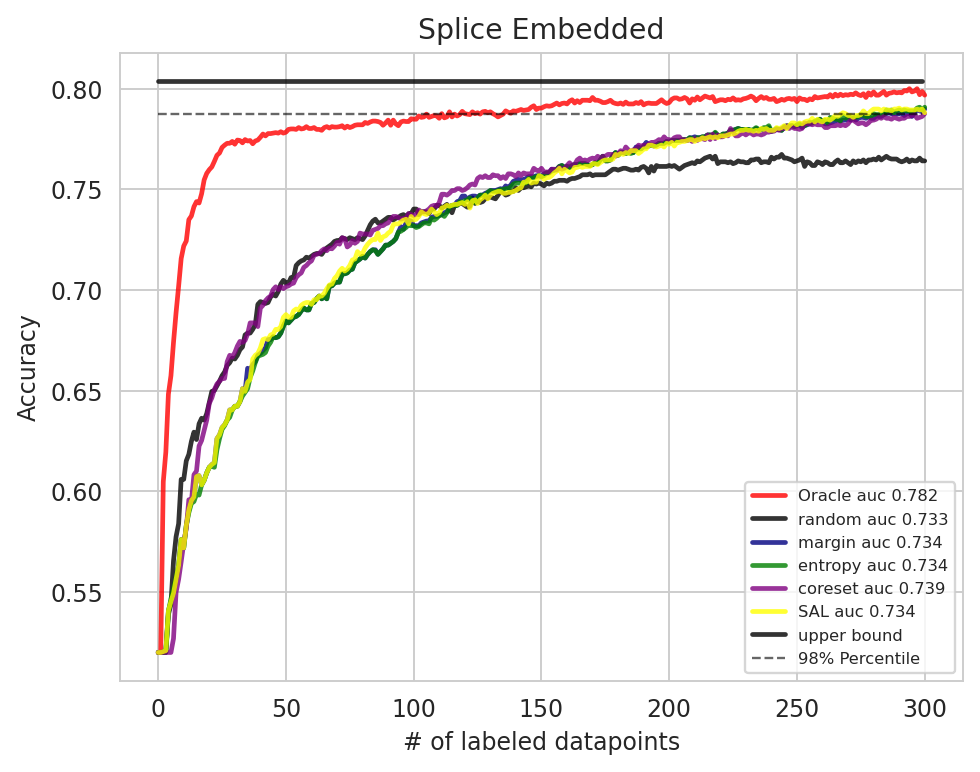
\includegraphics[width=0.8\linewidth]{img/eval_splice_embedded}
	\caption{Results for all algorithms on the pre-encoded Splice dataset}
\end{figure}
\begin{figure}[H]
\centering
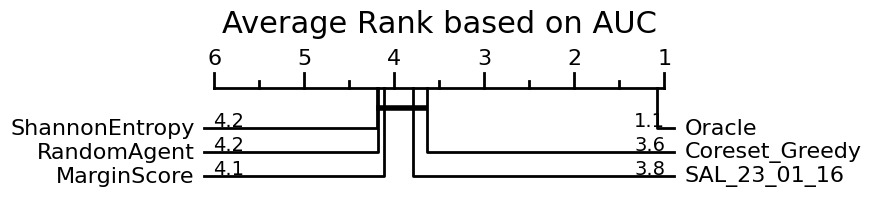
\includegraphics[width=0.8\linewidth]{img/eval_splice_embedded_cd}
\caption{Critical Difference Diagram for Splice where every restart of the algorithm is one sample for the Wilcoxon-Holm method}
\end{figure}
\begin{figure}[H]
\centering
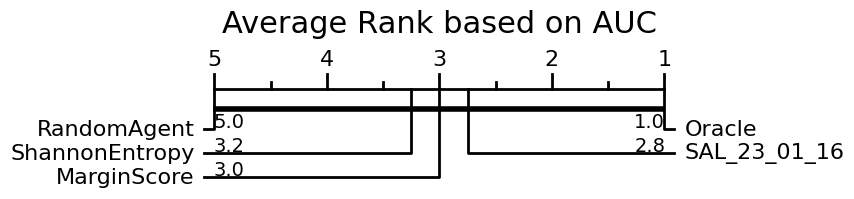
\includegraphics[width=0.8\linewidth]{img/eval_macro}
\caption{Critical Difference Diagram for Splice, DNA, USPS and Cifar10}
\end{figure}



%%%%%%%%%%%%%%%%%%%%%%%%%%%%%%%%%%%%%%%%%%%%%%%%%%%%%%%%%%%%%%%%%%%%%%%%%%%%%%%%%%
%%%%%%%%%%%%%%%%%%%%%%%%%%%%%%%%%%%%%%%%%%%%%%%%%%%%%%%%%%%%%%%%%%%%%%%%%%%%%%%%%%
\section{Ablation Studies}
\begin{itemize}
	\item Setting $\tau$ to $|\mathcal{U}|$
	\item Reduction of the test set for speed
\end{itemize}


\bibliographystyle{plain}
\bibliography{main.bib} 

\appendix


\section{Comparison of different sample sizes}
\begin{figure}[H]
	\centering
	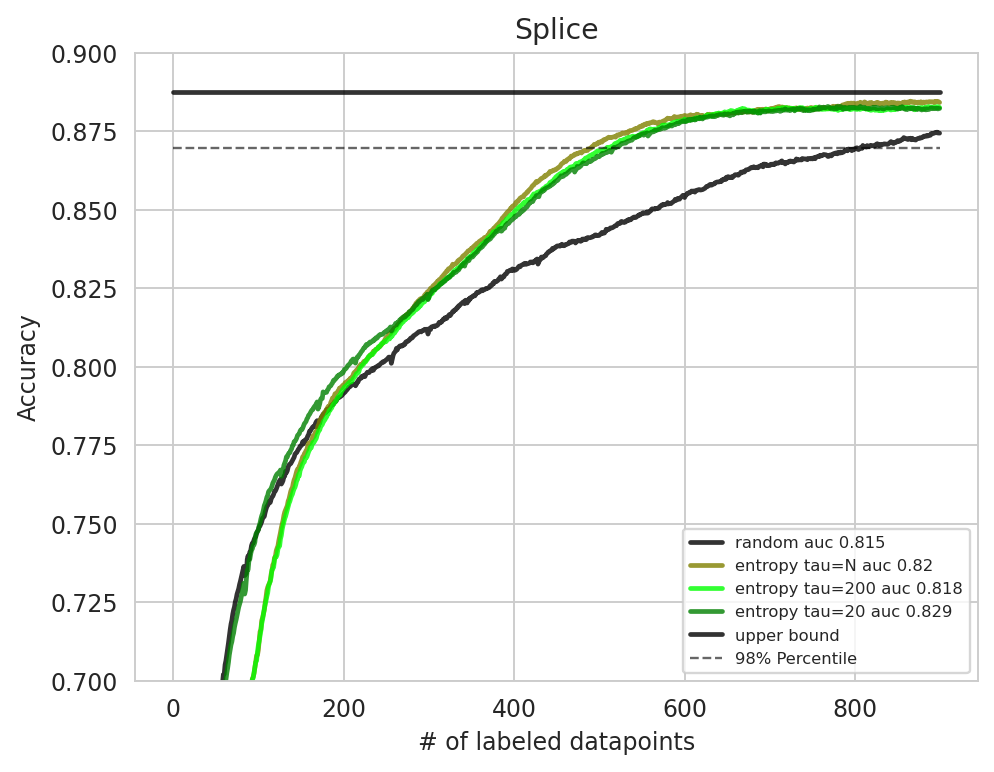
\includegraphics[width=0.7\linewidth]{img/tau_ablation.png}
\end{figure}

\end{document}
